\documentclass[11pt,a4paper]{article}

\usepackage{graphicx}
\usepackage{url}
\usepackage{listings}
\title{Accessing IO pins of port expander interfaced with R-Pi}
\author{e-Yantra Team}
\date{\today}

\begin{document}
	\maketitle
	\newpage
	\tableofcontents
	\newpage
	\section{Objective}
	In this tutorial we will learn to access IO pins of a port expander (MCP23017) interfaced with an R-Pi and will also perform some experiments with LED's, switches and LCD interfaced with this IC.
	\section{Prerequisites}
	\begin{itemize}
		\item Python programming skills
		\item An R-Pi (with I2C; I will be using version 2 ) 
		\item Interfacing an MCP23017 IC with an R-Pi should be known
	\end{itemize}
	
	\section{Hardware Requirement}
    \begin{enumerate}
    	\item Raspberry Pi (I will be using Version 2 Model B)
    	\item MCP23017
    	\item Power adapter
    	\item Connecting wires
    	\item LED's
    	\item 16x2 LCD display (I will be using model HD44780U)
    	\item Push button
    	\item Resistors (330 ohms)
    	\item Potentiometer (10k ohms)
    	\item Bread board
    \end{enumerate}
    
	\section{Software Requirement}
	\begin{enumerate}
		\item PyScripter (version 2.7 or above)
		\item Mobaxterm (for windows user)
	\end{enumerate}
	
	\newpage
	\section{Theory and Description}
	
	\textbf{16x2 LCD Display :}
	\vspace{0.3cm}
	\newline
	The HD44780U dot-matrix liquid crystal display controller and driver LSI displays alphanumerics,Japanese kana characters, and symbols. It can be configured to drive a dot-matrix liquid crystal display under the control of a 4- or 8-bit microprocessor. Since all the functions such as display RAM, character generator, and liquid crystal driver, required for driving a dot-matrix liquid crystal display are internally provided on one chip, a minimal system can be interfaced with this controller/driver.[3]
	\flushleft
	A 16x2 LCD means it can display 16 characters per line and there are 2 such lines. In this LCD each character is displayed in 5x7 pixel matrix. This LCD has two registers, namely, Command and Data. The \textit{Command} register stores the command instructions given to the LCD. A command is an instruction given to LCD to do a predefined task like initializing it, clearing its screen, setting the cursor position, controlling display etc. The \textit{Data} register stores the data to be displayed on the LCD. The data is the ASCII value of the character to be displayed on the LCD. [4]
	\vspace{0.3cm}
	\textbf{Pin Diagram}
    \begin{figure}[h!]
    	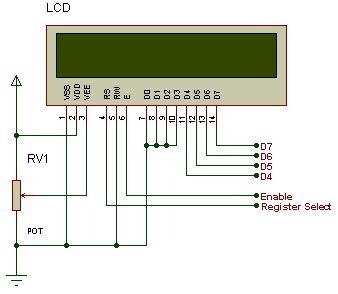
\includegraphics[scale=0.9]{lcd.png}
    	\centering
    	\caption{[5]}
    \end{figure} 
    	
	\newpage
	\flushleft
	\textbf{Pin Description }
	\vspace{0.3cm}
	
	\begin{tabular}{|c|c|c|}
		\hline
		Pin No & Function & Name \\
		\hline
		1 & Ground (0V) & Ground \\
		\hline
		2 & Supply voltage; 5V (4.7V – 5.3V) & Vcc \\
		\hline
		3 & Contrast adjustment; through a variable resistor & VEE \\
		\hline
		4 & Selects command register when low; and data register when high & Register Select \\
		\hline
		5 & Low to write to the register; High to read from the register & Read/write \\
		\hline
		6 & Sends data to data pins when a high to low pulse is given & Enable \\
		\hline
		7 & & DB0 \\
		\hline
		8 & & DB1 \\
		\hline
        9 & & DB2 \\
        \hline
		10 & 8-bit data pins & DB3 \\
		\hline
		11 & & DB4 \\
		\hline
		12 & & DB5 \\
		\hline
		13 & & DB6 \\
		\hline
		14 & &DB7 \\
		\hline
		15 & Backlight VCC (5V) & Led+ \\
		\hline
		16 & Backlight Ground (0V) & Led- \\
		\hline
	\end{tabular}
	\flushleft
	Ref: [4]
	
	
	\newpage
	\section{Experiments}
	\flushleft
	In order to program the MCP23017 chip (using I2C protocol) in Python you must install the \textbf{smbus} package. Once you have installed the package you can now start programming the chip.
    
    \vspace{0.3cm}
    \textbf{SMBus protocol commands:}
    \begin{itemize}
    	\item SMBus Read Byte:  i2c\_smbus\_read\_byte\_data()
    	This reads a single byte from a device, from a designated register.The register is specified through the Comm byte.
    	
    	S Addr Wr [A] Comm [A] S Addr Rd [A] [Data] NA P
    	
        \item SMBus Write Byte:  i2c\_smbus\_write\_byte\_data()
        
        This writes a single byte to a device, to a designated register. The register is specified through the Comm byte. This is the opposite of the Read Byte operation.
        
        S Addr Wr [A] Comm [A] Data [A] P
    	
    \end{itemize}
    
    \newpage
	\subsection{Interfacing an LED and a Switch to R-Pi using MCP23017 IC}
     \begin{figure}[h!]
     	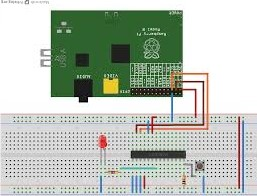
\includegraphics[scale=1.5]{i1.jpeg}
     	\centering
     	\caption{[2]}
     \end{figure} 
     
     As shown in the figure:
     \begin{itemize}
     	\item Pin 9 (VDD) is connected to 3.3V
     	\item Pin 10 (VSS) is connected to Ground
     	\item Pin 12 (SCL) is connected to Pin 5 on the Pi GPIO
     	\item Pin 13 (SDA) is connected to Pin 3 on the Pi GPIO
     	\item Pin 18 (Reset) should be set high for normal operation so we connect this to 3.3V
     	\item Pins 15, 16 \& 17 (A0-A2) determine the number assigned to this device. We are only using one device so we will give it a binary zero by setting all three of these pins to 0 (ground)
     	\item Led is connected to GPA0 and switch is connected to GPA7
     \end{itemize}
    
    \newpage 
    \textbf{Code}
    \vspace{0.3cm}
    
    \lstinputlisting[language=Python]{i2cls.py}
    
    \newpage 
	\subsection{Interfacing an LCD to an R-Pi using MCP23017 IC}
	\begin{figure}[h!]
		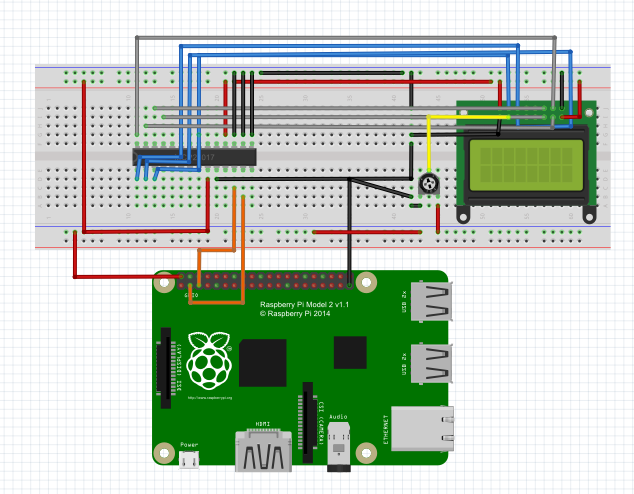
\includegraphics[scale=0.7]{i2.PNG}
		\centering
		\caption{[2]}
	\end{figure} 
	
	 As shown in the figure:
	 \begin{itemize}
	 	\item Pin 9 (VDD) is connected to 5V (Red)
	 	\item Pin 10 (VSS) is connected to Ground (Black)
	 	\item Pin 12 (SCL) is connected to Pin 5 on the Pi GPIO (Orange)
	 	\item Pin 13 (SDA) is connected to Pin 3 on the Pi GPIO (Orange)
	 	\item Pin 18 (Reset) should be set high for normal operation so we connect this to 5V (Red)
	 	\item Pins 15, 16 \& 17 (A0-A2) determine the number assigned to this device. We are only using one device so we will give it a binary zero by setting all three of these pins to 0 (ground) (Black)
	 	\item RS,RW and Enable pins of the LCD are connected to GPB0,GPB1 and GPB2 respectively.
	 	\item Data pins D7,D6,D5 and D4 are connected to GPS7,GPA6,GPA5 and GPA4 respectively.
	 \end{itemize}
	
	\newpage 
	\textbf{Code}
	\vspace{0.3cm}
	
	\lstinputlisting[language=Python]{i2clcd.py}
	
	\vspace{0.3cm}
	\textbf{Note:} This code can be imported into any other python code for further usage (eg: for displaying sensor values on lcd).
	
	\newpage
	\section{Appendix}
	
	\subsection{Raspberry Pi 2 Pin-out Diagram}
	\begin{figure}[h!]
		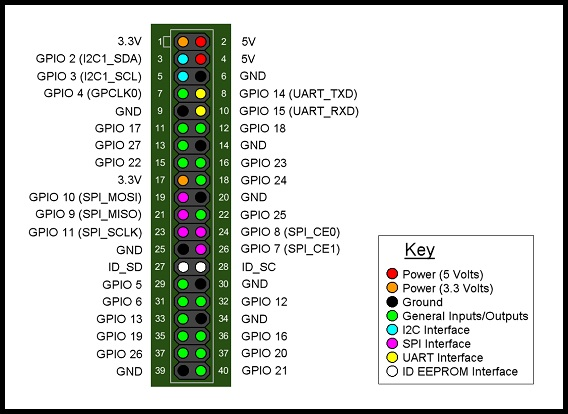
\includegraphics[scale=0.6]{RaspberryPi2_pinout.jpg}
		\centering
		\caption{[5]}
	\end{figure}
			
	\subsection{MCP23017 datasheet}
			
	\url{http://ww1.microchip.com/downloads/en/DeviceDoc/21952b.pdf}
			
	\newpage
	\section{References}
	\begin{enumerate}
		\item \url{https://www.kernel.org/doc/Documentation/i2c/smbus-protocol}
		\item \url{http://dangerousprototypes.com/wp-content/media/2013/04/mcp23017test_bb-600x458.png}
		\item \url{https://www.sparkfun.com/datasheets/LCD/HD44780.pdf}
		\item \url{http://www.engineersgarage.com/electronic-components/16x2-lcd-module-datasheet}
		\item \url{http://data.designspark.info/uploads/images/53bc258dc6c0425cb44870b50ab30621}
    \end{enumerate}
	
\end{document}



